% Time-memory-data cryptanalysis of the HiTag2 stream cipher
%
% Presentation file
% Rajesh Bachani

\documentclass{beamer}
\setbeamertemplate{navigation symbols}{}

\usepackage[english]{babel}
\usepackage[latin1]{inputenc}
\usepackage{graphicx}
\usepackage{colortbl}
\usepackage{url}
\usepackage{beamerthemeshadow}
\usepackage[english]{babel}
% or whatever

\usepackage[latin1]{inputenc}
% or whatever

\mode<presentation>
{
  \usetheme{Warsaw}
  % or ...

  \setbeamercovered{transparent}
  % or whatever (possibly jweust delete it)
}

% Delete this, if you do not want the table of contents to pop up at
% the beginning of each subsection:
\AtBeginSubsection[]
{
	\begin{frame}<beamer>{Outline}
  \footnotesize{  \tableofcontents[currentsection,currentsubsection]}
  \end{frame}
}

% If you wish to uncover everything in a step-wise fashion, uncomment
% the following command: 

%\beamerdefaultoverlayspecification{<+->}


% the document begins here

\begin{document}
\title{Time-memory-data cryptanalysis of the HiTag2 stream cipher}
\subtitle{M.Sc. project presentation}

\author{Rajesh Bachani}

\institute
{
  Department of Mathematics\\
  Technical University of Denmark
}

\date
{
	Supervisor: Dr.~Erik Zenner
}

\begin{frame}
  \titlepage
\end{frame}

\begin{frame}{Outline}
  \footnotesize{\tableofcontents}
\end{frame}

\section{Introduction}

\subsection{Basics}

\begin{frame}{Cryptography}
\footnotesize{
  \begin{itemize}
  \item Cryptography provides data confidentiality, integrity, authentication, non-repudiation etc. 
  \item Main ideas: encryption, decryption and `secret key'
  \item Cryptosystems can be symmetric-key or asymmetric-key
  \item Symmetric-key cryptosystems are further divided into two categories: 
  	\begin{itemize}
  	\footnotesize{
			\item Block cipher
  		\item Stream cipher}
  	\end{itemize}
  \end{itemize}}
\end{frame}

\begin{frame}{One-time pad}
\footnotesize{
  \begin{itemize}
  \item OTP provides the basic design principle for stream ciphers
  \item A random key is chosen and \textit{xor}'ed with plaintext, bitwise
  \end{itemize}
  
  \begin{figure}[htp]
	\centering
	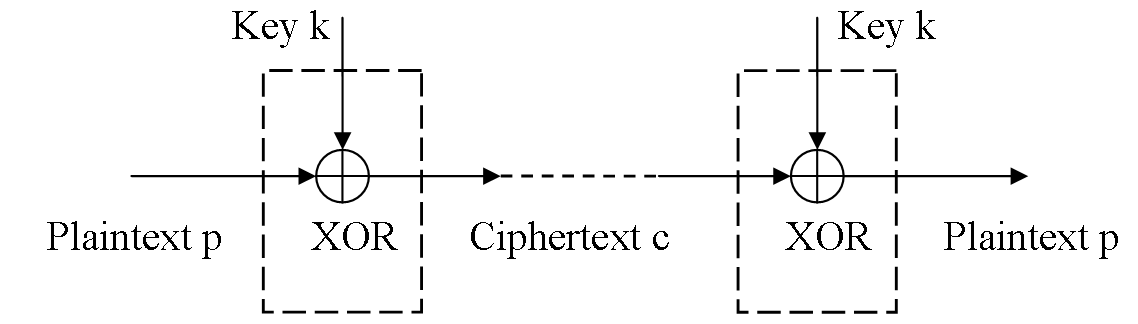
\includegraphics[width = 3in]{./figures/one-time-pad.PNG}
	\end{figure}
	
	\begin{itemize}
		\item Provided the key is truly random, OTP exhibits perfect secrecy
		\item Practically, suffers from the following problems:
  	\begin{enumerate}
  		\footnotesize{
  		\item Long and random key is required
  		\item Key can be used just once}
  	\end{enumerate}
  \end{itemize}}
\end{frame}


\begin{frame}{Pseudo-random number generator}
	
	\footnotesize{
	\begin{itemize}
		\item PRSG generates a long pseudo-random \textit{keystream} using a short key
		\item The same key can be re-used by using a different initialization parameter for every run of the cipher
	}\end{itemize}
	
  \begin{figure}[htp]
	\centering
	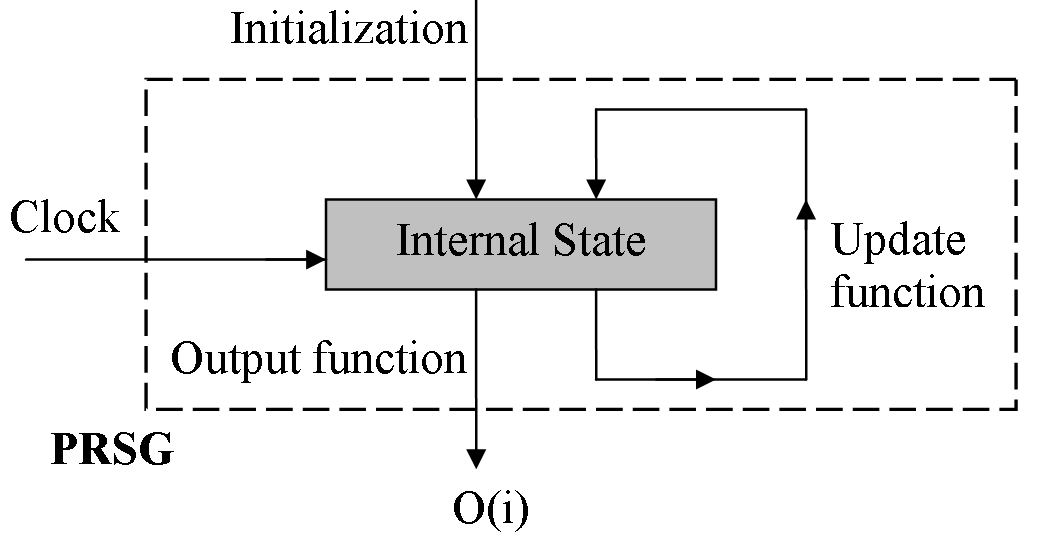
\includegraphics[width = 2.5in]{./figures/prsg.PNG}
	\end{figure}

\end{frame}

\begin{frame}{Linear feedback shift register}
	\footnotesize{
	\begin{itemize}
		\item Linear feedback shift register (LFSR) is one way to implement PRSG
		\item Two components: shift register and linear feedback function
	\end{itemize}
	}
	\begin{columns}
	
	\begin{column}{6cm}
	\begin{figure}[htp]
	\centering
	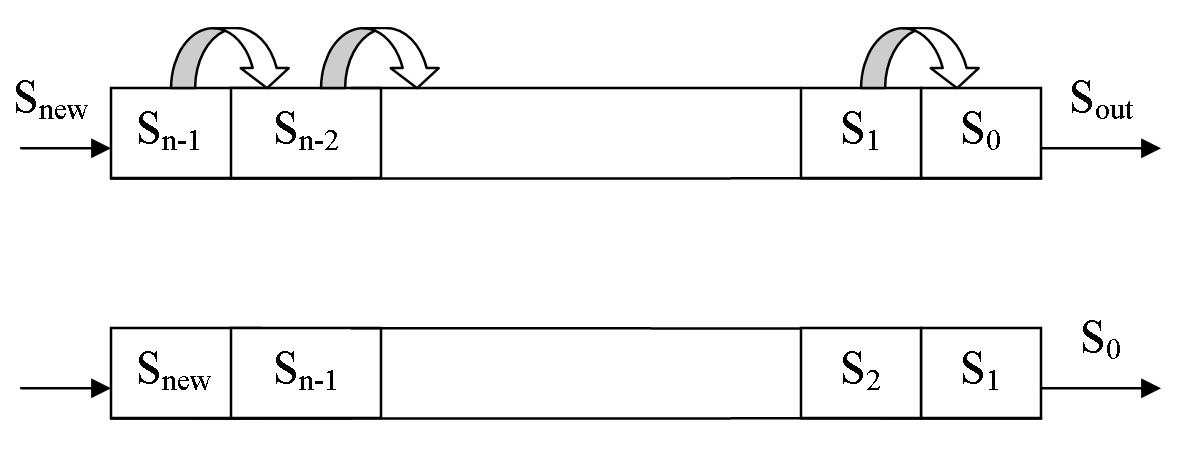
\includegraphics[width = 1.8in]{./figures/shift-register.PNG}
	\end{figure}
	\end{column}
	
	\begin{column}{6cm}
	\begin{figure}[htp]
	\centering
	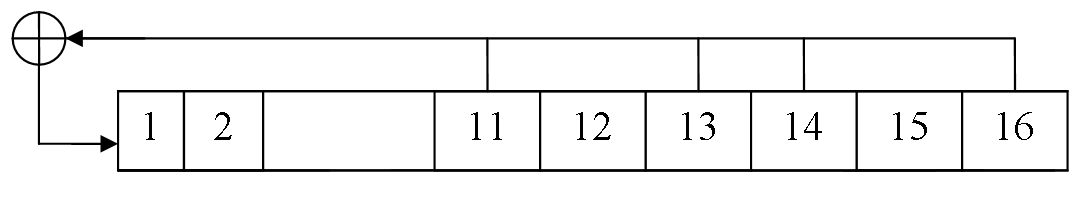
\includegraphics[width = 1.8in]{./figures/lfsr-example.PNG}
	\end{figure}
	\end{column}	

	\end{columns}

	\begin{columns}
	\begin{column}{6cm}
	\footnotesize{
	\begin{itemize}
		\item Bits 11, 13, 14 and 16 are called \emph{tap} bits
		\item Cycle of generated states should be maximal ($2^n - 1$)
		\item Well chosen tap sequence gives maximal length cycle of states
	\end{itemize}}
	\end{column}	
	
	\begin{column}{6cm}
	\begin{figure}[htp]
	\centering
	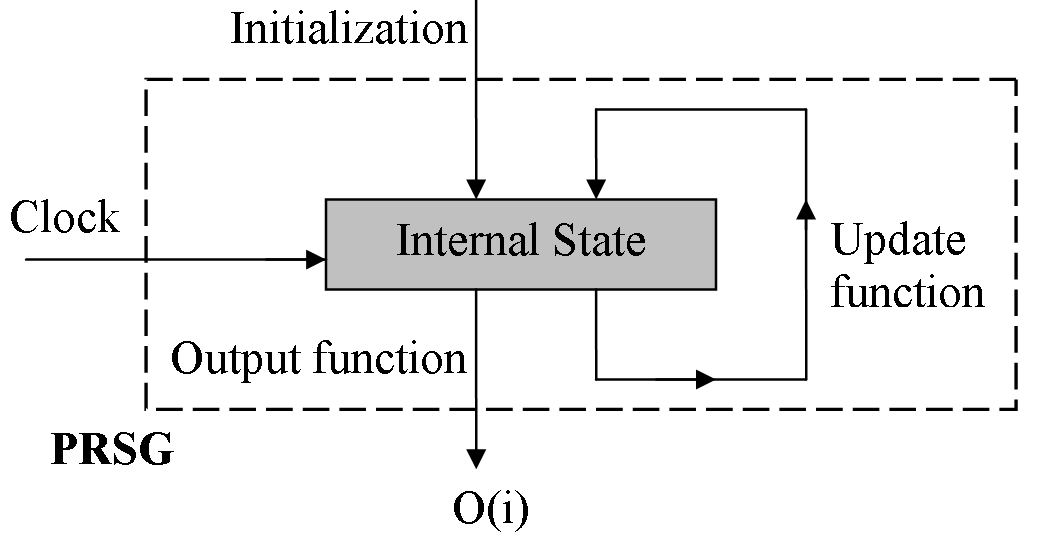
\includegraphics[width = 1.9in]{./figures/prsg.PNG}
	\end{figure}
	\end{column}	
	\end{columns}	
\end{frame}	

\begin{frame}{Internal model of stream cipher}

  \begin{figure}[htp]
	\centering
	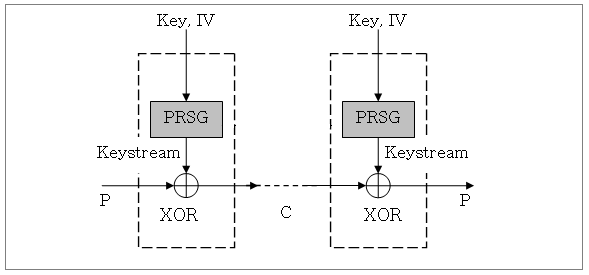
\includegraphics[width = 2.2in]{./figures/stream-cipher.PNG}
	\end{figure}

	\begin{itemize}
		\footnotesize{\item The perfect secrecy of OTP does not apply here as the keystream is pseudo-random in nature}
	\end{itemize}
\end{frame}


\subsection{Time-memory tradeoff attacks}

\begin{frame}{Time-memory tradeoff}
\begin{itemize}
\footnotesize{	
	\item Consider a block cipher with key length $k$; known-plaintext scenario for attacker
	\item Brute force attack: try all possible keys
		\begin{itemize}
			\footnotesize{\item Takes $2^k$ operations in time; no memory required}
		\end{itemize}
	\item Precomputed ciphertext attack: store all possible ciphertexts along with keys
		\begin{itemize}
			\footnotesize{\item Takes constant operation in time; $2^k$ memory required}
		\end{itemize}
	\item Time-memory tradeoff attack: time and memory requirements are reduced from the two extremes
}\end{itemize}

\end{frame}

\begin{frame}{Other important concepts}
\begin{itemize}
\footnotesize{	
	\item Birthday paradox:
	\begin{itemize}
	\footnotesize{	
		\item If 23 people are present in a single room, 50\% chances of two people having same birthday
		\item Variant: If 17 people each are present in two rooms, 50\% chances of two people in different rooms having the same birthday
		\item Variant considers two sets and determines probability for a common element between these two sets\\
		\begin{center}
			$P(m, n_1, n_2) = 1 -(1 - n_2/m)^{n_1}$\\
		\end{center}
		\item For $P(m, n_1, n_2) \approx 1$ and $m \rightarrow \infty$
		\begin{center}
			$n_1 \cdot n_2 \geq m$
		\end{center}
	}\end{itemize}

	\item Hashtable:
	\begin{itemize}
	\footnotesize{	
		\item Allow searching in constant time
		\item Every \emph{hashvalue} has to have a unique identifier called \emph{hashkey}
	}\end{itemize}
	
}\end{itemize}
		


\end{frame}

\subsection{HiTag2 stream cipher}

\begin{frame}{Background}
\begin{itemize}
\item HiTag2 stream cipher is used for remote keyless entry in cars by providing two-way authentication between car and car key
\item It was a proprietary algorithm of Philips Semiconductors (now NXP)
\item HiTag2 was reverse-engineered from its software implementation recently
\end{itemize}
\end{frame}

\begin{frame}{Design}
\begin{itemize}
	\item Components of HiTag2:
	\begin{itemize}
		\item 48 bit key
		\item 32 bit serial ID
		\item 32 bit initialization vector (IV)
		\item 48 bit internal state with linear update function (basically, an LFSR)
		\item Non-linear output function based on multiplexor
	\end{itemize}
	
	\item Cipher is initialized in the following three phases:
	\begin{itemize}
		\item LFSR initialization
		\item LFSR setup
		\item Keystream generation
	\end{itemize}

\end{itemize}
\end{frame}

\begin{frame}{LFSR initialization and setup}
\begin{itemize}
	\item \small{Internal state is initialized using the serial ID and least significant 16 bits of secret key}
\end{itemize}
	\begin{figure}[htp]
	\centering
	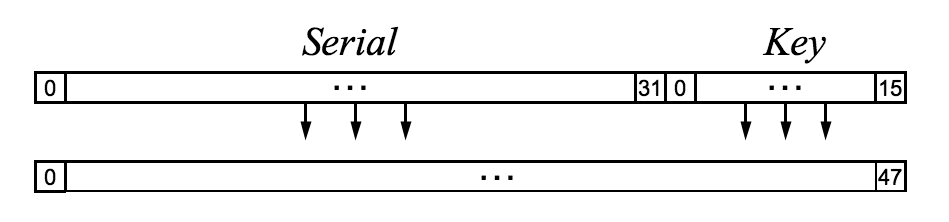
\includegraphics[width = 2in]{./figures/hitag2-1.PNG}
	\end{figure}
\begin{itemize}
		\item \small{During setup, one bit each from the key, the IV and the output are \textit{xor}'ed and result is used as new bit for the internal state}
\end{itemize}

	\begin{figure}[htp]
	\centering
	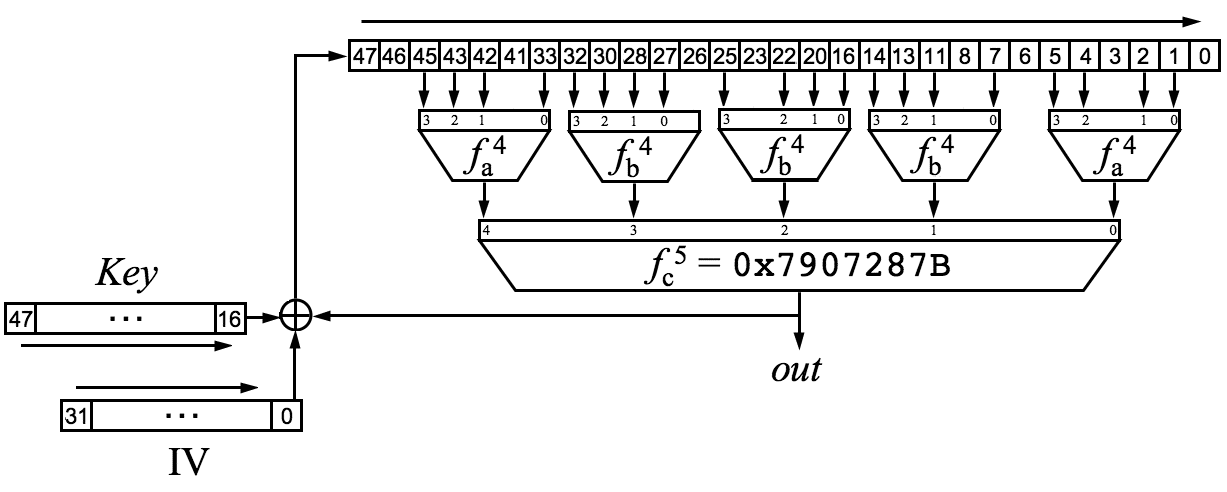
\includegraphics[width = 2.95in]{./figures/hitag2-2.PNG}
	\end{figure}
	
\end{frame}

\begin{frame}{Output function}

	\begin{figure}[htp]
	\centering
	\includegraphics[width = 2.5in]{./figures/output-function.PNG}
	\end{figure}
	
	\begin{figure}[htp]
	\centering
	\includegraphics[width = 3.2in]{./figures/table-mux.PNG}
	\end{figure}

\end{frame}

\begin{frame}{Keystream generation}
\begin{itemize} 
	\item Bit numbers 0, 2, 3, 6, 7, 8, 16, 22, 23, 26, 30, 41, 42, 43, 46 and 47 are used as \textit{tap} bits for updating the state
	\item Output of multiplexor $f_c^5$ constitutes the keystream bit
\end{itemize}

	\begin{figure}[htp]
	\centering
	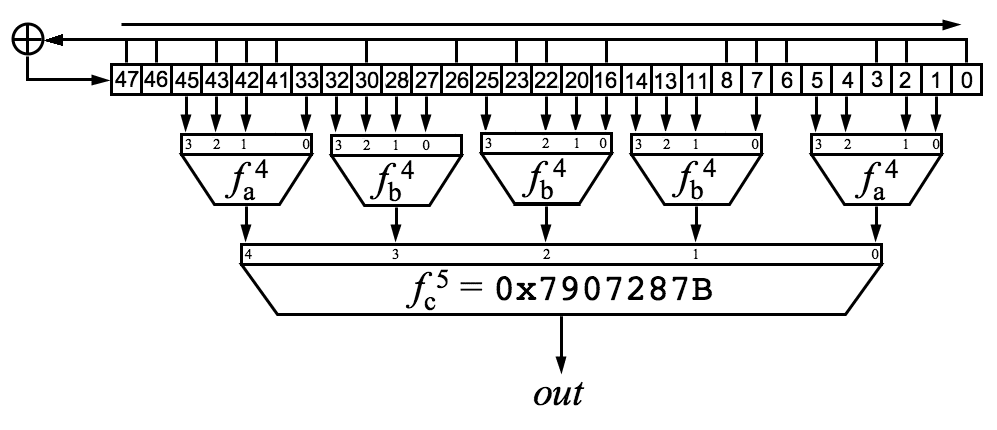
\includegraphics[width = 3in]{./figures/hitag2-3.PNG}
	\end{figure}

\end{frame}

\subsection{Motivation}
\begin{frame}{Motivation}
\begin{itemize}
	\item The internal state of HiTag2 is 48 bits
	\item A brute-force attack takes time of the order of $2^{48}$
	\item With the availability of a few hundred MB's of RAM, a time-memory tradeoff attack should be able to break HiTag2 on a PC
\end{itemize}
\end{frame}

\section{Babbage Golic time-memory tradeoff}

\subsection{Babbage Golic attack}

\begin{frame}{Basic idea of the attack}
\begin{itemize}
\small{
	\item Goal: to find one of the several occuring values of the internal state
}
\end{itemize}
	
	\begin{figure}[htp]
	\centering
	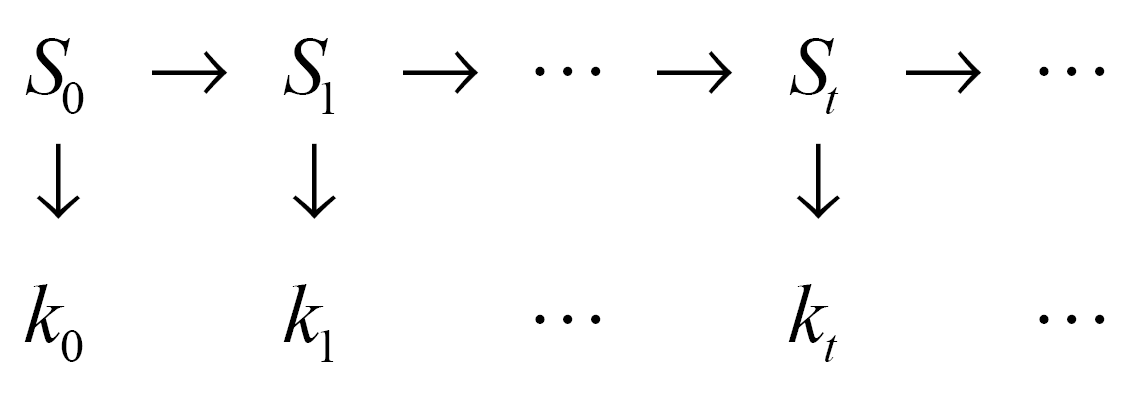
\includegraphics[width = 1.7in]{./figures/prsgmodel.PNG}
	\end{figure}

\begin{itemize}	
\small{
	\item The output sequence of certain length from a state (called \textit{prefix}) unique to that state
	\item Precomputation phase: $n_1$ states are randomly chosen, their prefix computed and stored
	\item Attack phase: subsequences of keystream (each corresponding to one of the $n_2$ states occuring) are matched with prefixes stored in memory
	\item According to the birthday paradox: $n_1 \cdot n_2 \geq 2^n$
}
\end{itemize}
\end{frame}

\begin{frame}{Parameters and tradeoff equation}

\begin{itemize}
\small{	
	\item Following parameters are used to define any tradeoff attack:
	\begin{itemize}
	\item \emph{M} represents the order of memory size required
	\item \emph{P} represents the order of time required for the precomputation phase
	\item \emph{T} represents the order of time required for the attack phase
	\item \emph{D} represents the order of prefixes available during the attack phase
	\end{itemize}
	\item \emph{M} is same as $n_1$, and \emph{T} is same as $n_2$; then we have the following tradeoff equation: $M \times T \geq 2^n$
}
\end{itemize}
\end{frame}

\begin{frame}{Attack with non-random precomputation}
\begin{itemize}
\small{
	\item Precomputation phase:
	\begin{itemize}
	\item States are not selected at random now
	\item Goal: to store states occurring at equidistant points in the huge cycle of internal states
	\item The distance between each state is then $d = 2^n/M$	
	\item An initial state $S_{initial}$ is randomly selected, and subsequenct states $S_{initial+d}$, $S_{initial+2d}$ are computed

	\end{itemize}
	\item Attack phase:
	\begin{itemize}
		\item If $d$ states occur in the keystream, then we can be sure that atleast one state would match in the memory
		\item Hence, $T$ =  $d$
	\end{itemize}
	\item Tradeoff equation:
	\begin{itemize}
		\item We can then deduce: $M \times T = 2^n$
		\item Note the difference with the tradeoff equation for random precomputation
	\end{itemize}
	
}	
\end{itemize}
\end{frame}

%\begin{frame}{State transition function}
%\small{
%\begin{itemize}
%	\item If $U$ represents the update function matrix, then the next state can be computed from curent state using the matrix multiplication: $S_{next}$ = $U . S_{current}$
%	\item State transition function $A$ returns the state occurring $d$ states after a given state by:\\
%	$S_{current + d}$ = $A . S_{current}$, such that $A = \underbrace{U . U . U \dots U}_{d}$
%	\item An efficient way to compute matrix $A$ is: $A = \underbrace{(((U^2)^2) \dotsc )^2}_{\log_2{d}}$
%	\item $A$ is computed just once in this fashion for the precomputation, and further states are computed as:\\
%	$S_{current + 2d}$ = $A . S_{current + d}$, \\$S_{current + 3d}$ = $A . S_{current+2d}$ $\dots$
%\end{itemize}
%}
%\end{frame}

\begin{frame}{Implementation}
\small{
\begin{itemize}
	\item The implementation is done in C language and the attack program run on shared Sun Solaris machine
	\item Results are produced for two different keys $K_1$ and $K_2$
	\item Prefix of length 48 bits and 56 bits are chosen
	\item A random number generator is implemented using the C rand() function, which gives a period of $2^{27}$ for generating 48 bit states for random precomputation
\end{itemize}
}
\end{frame}


\begin{frame}{Results}
	\begin{figure}[htp]
	\centering
	\includegraphics[width = 3.1in]{./figures/table-tmto-keystream-1.PNG}
	\end{figure}

\begin{itemize}
\small{	\item Column 3-4: In column 3, the key is not found. If $M$ is doubled, key is found two times.
	\item Column 7-8: In column 7, $M \times T = 2^{48}$; correct key is found exactly once as expected. If either $M$ or $T$ is doubled, the key is found exactly two times.}  
\end{itemize}

\end{frame}

\begin{frame}{Results}
	\begin{figure}[htp]
	\centering
	\includegraphics[width = 3.1in]{./figures/table-tmto-keystream-1.PNG}
	\end{figure}
\begin{itemize}
\small{
	\item Column 6: Correct key is found even if $M \times T < 2^{48}$. This does not occur always.
	\item Prefix length 48 bits gives false keys, whereas prefix length 56 bits gives no false keys. This shows that 48 bits of keystream is not sufficient to identify an internal state uniquely. }

\end{itemize}
\end{frame}

\subsection{Babbage Golic attack with short keystream}

\begin{frame}{Basic idea of the attack}
\small{
\begin{itemize}
	\item 32 bit keystream is exchanged between car key and controller for authentication (\emph{authenticator tag})
	\item Attacker has several authenticator tags
	\item Precomputation: 
	\begin{itemize}
		\item $M$ internal states are chosen in non-random fashion and their tags computed and stored
	\end{itemize}
	\item Attack: 
	\begin{itemize}
		\item Attacker has $T$ random IV's and the corresponding tags
		\item If the tag is found in memory, find the secret key using the initial state corresponding to the tag
		\item Keep on matching and finding secret keys, until one of the secret key repeats
	\end{itemize}
\end{itemize}
}
\end{frame}

\begin{frame}{Probability of finding the key}
\begin{itemize}
\small{
	\item Probability of matching a tag in memory $P_1$ = $M/2^{32}$
	\item Probability of a matched tag giving the correct initial state (thus the correct key) $P_2$ = $2^{32}/2^{48}$
	\item Overall probability of finding the secret key $P$ = $P_1 \cdot P_2$ = $M/2^{48}$
	\item If $T$ tags are known, the probability of finding the correct key once is $M/2^{48} \cdot T$
	\item Tradeoff equation: $M \cdot T \geq 2^{48}$
%	\item If $M \cdot T \geq 2 \cdot 2^{48}$, correct key is expected to be found twice; \\if $M \cdot T \geq 4 \cdot 2^{48}$, correct key is expected to be found four times, etc
}
\end{itemize}
\end{frame}

\begin{frame}{Results}

	\begin{figure}[htp]
	\centering
	\includegraphics[width = 3.1in]{./figures/table-tmto-tags.PNG}
	\end{figure}
\begin{itemize}
\scriptsize{
	\item The number of tags matching is around the expected value. They are slightly higher since many states can result in same tag during the attack phase.
	\item In column 2 for key $K_2$, key is not found even once. In column 3, the key is found four times as expected. This can be clearly attributed to the probabilistic nature of the tradeoff equation.
}
\end{itemize}
\end{frame}


\section{Time-memory-data tradeoff using Hellman tables}

\subsection{Hellman tables for block ciphers}

\begin{frame}{Ideal Hellman tables}
\footnotesize{
	\begin{columns}
	\begin{column}{5cm}
	\begin{itemize}
		\item Block cipher encryption denoted by $C$ = $E_K(P)$
		\item $P$ and $C$ are known to attacker, $K$ is to be found
	\end{itemize}
	\end{column}
	
	\begin{column}{5cm}
	\begin{figure}[htp]
	\centering
	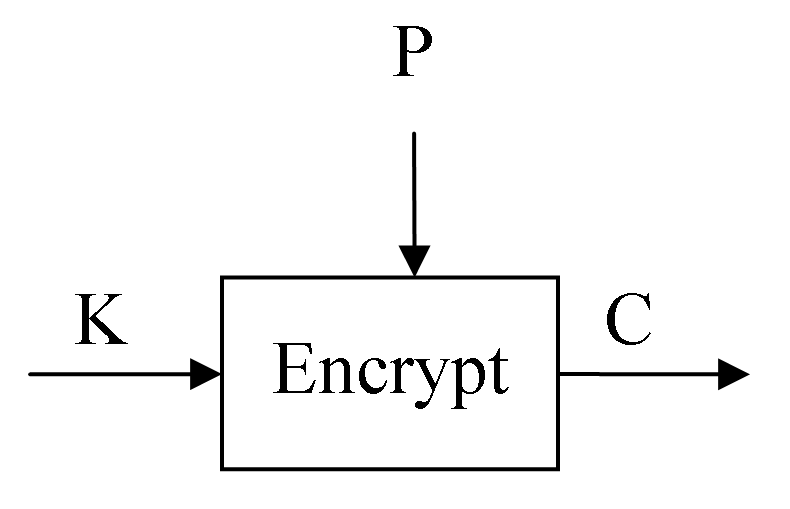
\includegraphics[width = 1.1in]{./figures/block-cipher.PNG}
	\end{figure}
	\end{column}

\end{columns}	

\begin{itemize}
\item Precomputation phase:
\begin{itemize}
	\item A starting point $K_0$ is randomly chosen
	\item A chain is a sequence of encryptions which use ciphertext from the previous encryption as key for the next encrytion
\end{itemize}

	\begin{figure}[htp]
	\centering
	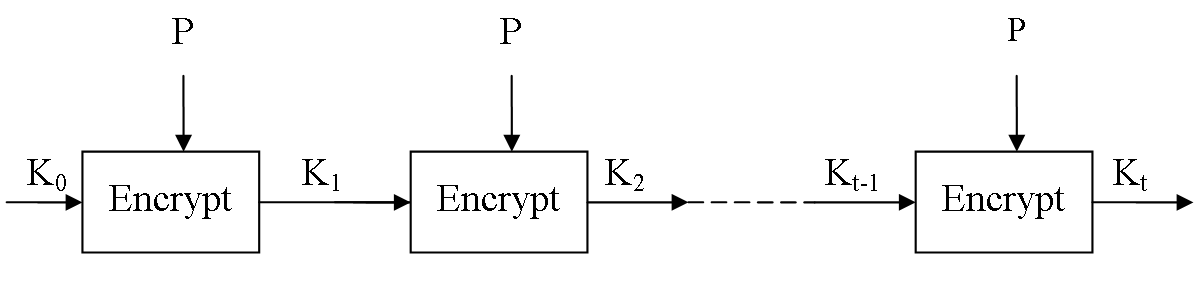
\includegraphics[width = 2.7in]{./figures/block-cipher-single-chain.PNG}
	\end{figure}

\begin{itemize}
	\item $m$ such chains are created
\end{itemize}
\end{itemize}
}
\end{frame}

\begin{frame}{Ideal Hellman tables}
\footnotesize{
	\begin{figure}[htp]
	\centering
	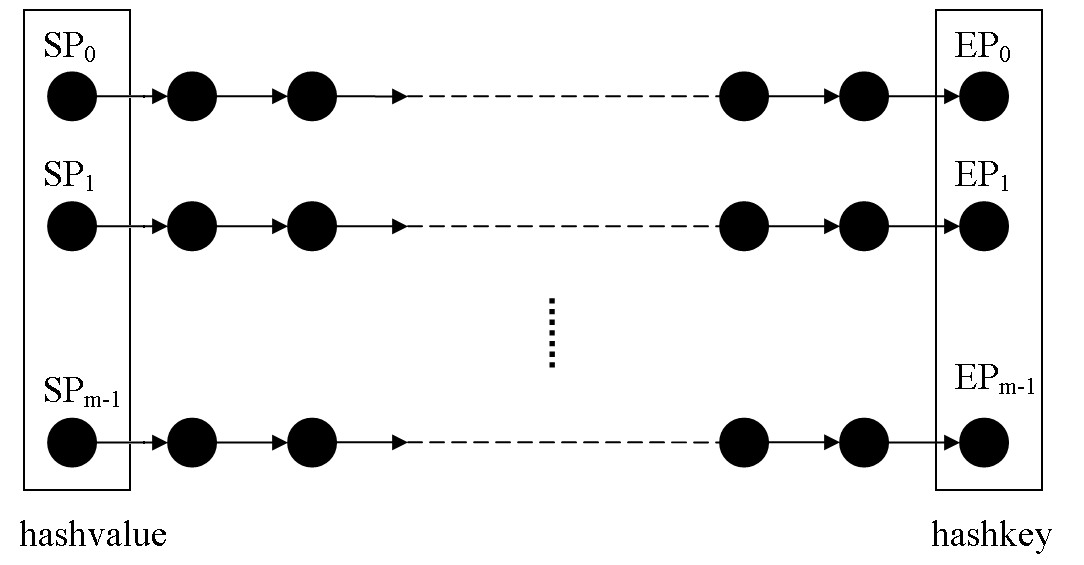
\includegraphics[width = 3in]{./figures/naive-hellman-table.PNG}
	\end{figure}

\begin{itemize}
	\item Tradeoff parameters: $M$ = $m$; $P$ = $mt$ = $2^k$ (Note that $M \neq P$)
	\item Attack phase:
	\begin{itemize}
	\footnotesize{
		\item $C$, $E_C(P)$, $E_{E_K(C)}(P)$, $\dots$ are matched with EP
		\item Worst case runtime in the order of length of the chain or $t$
	}
	\end{itemize}
\end{itemize}
}
\end{frame}

\begin{frame}{Problems and solution}
\footnotesize{
\begin{enumerate}
	\item Block length of cipher and key size are not always equal\\
	Solution: Use \emph{mapping function}
	\begin{figure}[htp]
	\centering
	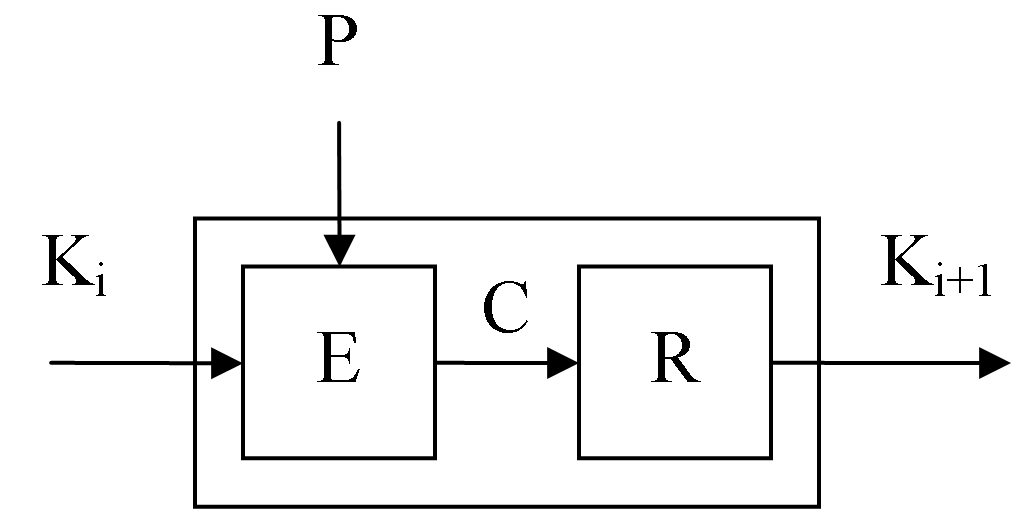
\includegraphics[width = 1.2in]{./figures/mapping-function.PNG}
	\end{figure}
	\item As the table grows, keys would start repeating resulting in collision and merging of distinct chains
	\begin{itemize}
	\footnotesize{
		\item Precomputation phase: wastage of memory and time
		\item Attack phase: false alarms
	}
	\end{itemize}
	\begin{columns}
	
	\begin{column}{5cm}
	\begin{figure}[htp]
	\centering
	Collision and merge
	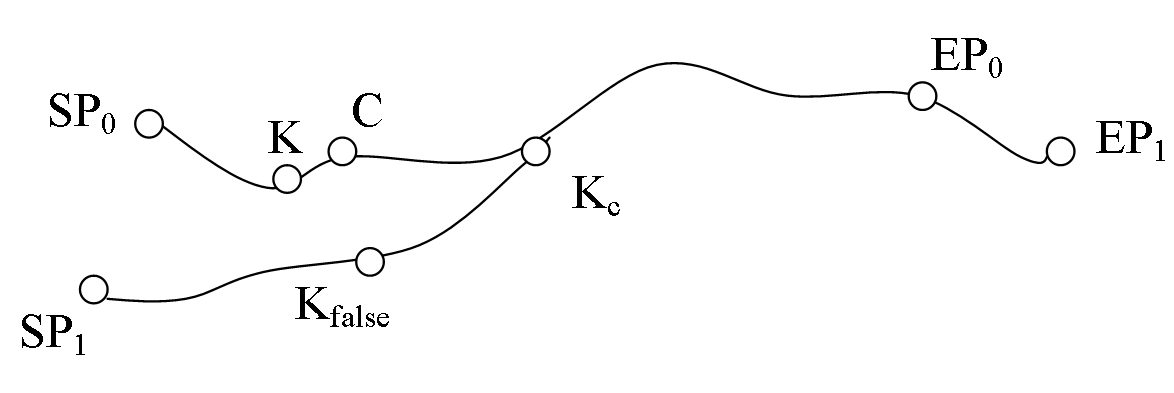
\includegraphics[width = 2.1in]{./figures/collision-merge.PNG}
	\end{figure}
	\end{column}
	\begin{column}{5cm}
	\begin{figure}[htp]
	\centering
	Collision but no merge
	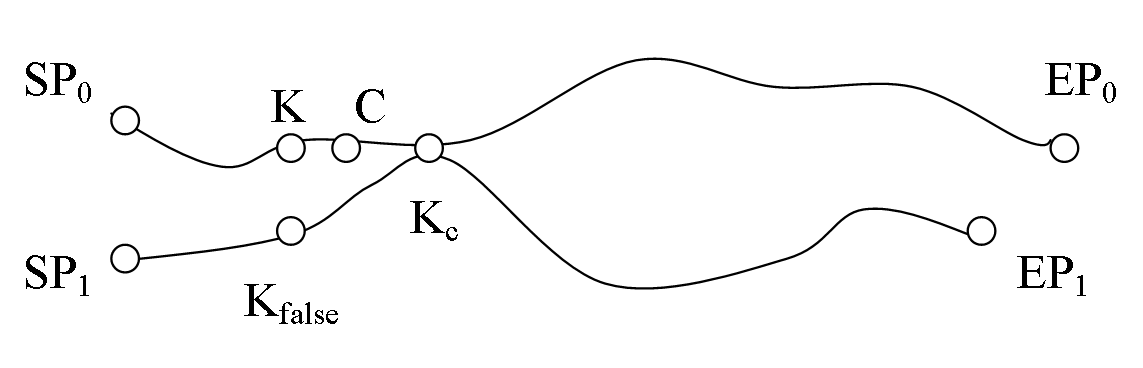
\includegraphics[width = 2.1in]{./figures/collision-not-merge.PNG}
	\end{figure}
	\end{column}
	\end{columns}	
\end{enumerate}
}
\end{frame}

\begin{frame}{Practical Hellman tables}
\begin{columns}
\begin{column}{7cm}
\footnotesize{
\begin{itemize}
	\item There are multiple tables; $r$ denotes the number of tables
	\begin{itemize}
	\footnotesize{
		\item Number of keys in each table is restricted using the \emph{table stopping rule}
		\item Rule: $mt \cdot t \leq 2^k$
	}
	\end{itemize}
	\item Each table has a different reduction function
	\item Tradeoff parameters: \\
	\begin{center}$M$ = $mr$ \\$P$ = $mtr$ = $2^k$ \\$T$ = $rt$\\ $r = t$ \end{center}
\end{itemize}
}
\end{column}

\begin{column}{6cm}
	\begin{figure}[htp]
	\centering
	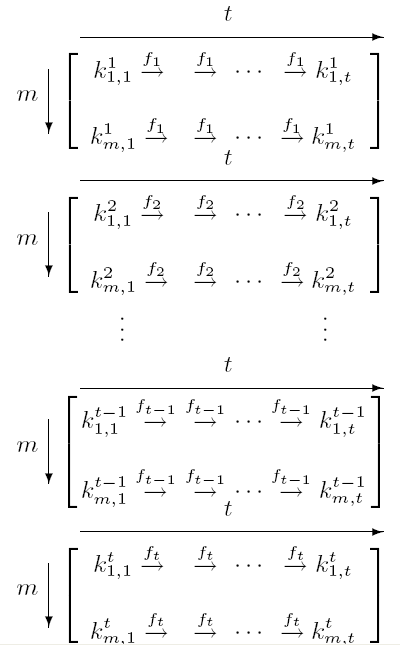
\includegraphics[width = 1.6in]{./figures/hellman-tables.PNG}
	\end{figure}

\end{column}

\end{columns}
\end{frame}

\subsection{Hellman tables for stream ciphers}
\begin{frame}{Modifications for stream ciphers}
\begin{itemize}
\footnotesize{
	\item Modification 1: key is replaced by internal state and ciphertext by prefix. The mapping function becomes:
	\begin{figure}[htp]
	\centering
	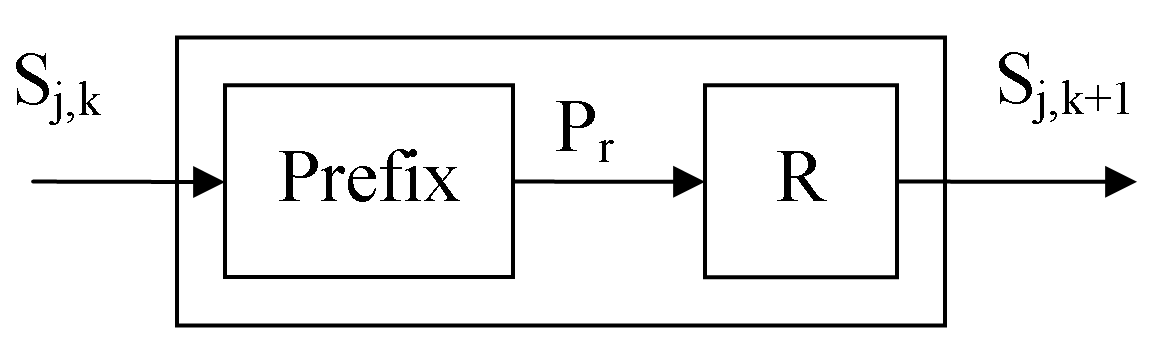
\includegraphics[width = 1.5in]{./figures/mapping-function-stream.PNG}
	\end{figure}
	\item Modification 2: since several internal states occur in available keystream, $P$ can be reduced. From birthday paradox:\\
	$P \cdot D \geq mtr$, thus $P = mtr/D$
	\begin{itemize}
	\footnotesize{
		\item Two possibilities: reduce number of tables or reduce number of states in each table
		\item According to Biryukov-Shamir, number of tables should be reduced by $D$
	}\end{itemize}
	\item 

}
\end{itemize}
\end{frame}

\begin{frame}{A general tradeoff equation}
\begin{itemize}
	\item In Biryukov-Shamir tradeoff, $r$ depends on $D$; implying a precomputation phase parameter depends on an attack phase parameter
	\item To avoid this dependency, we consider the general tradeoff equation:\\
	\begin{center}
	$mtr \cdot D = 2^n$
	\end{center}
\end{itemize}
\end{frame}


\subsection*{Implementation results}
\begin{frame}{Implementaton results}
\begin{columns}
\begin{column}{4cm}
\begin{itemize}
\scriptsize{
	\item With general tradeoff equation, parameters can be chosen independent of each other
	\item On increasing the number of tables, false alarms decrease proportionally
	\item This shows that the \emph{table stopping rule} does not provide correct upper bounds (column 4 and 6)
	\item Tradeoff equation does not guarantee the key to be found, it is probabilistic (column 4, 5 and 7)
	
}\end{itemize}
\end{column}
\begin{column}{7cm}
	\begin{figure}[htp]
	\centering
	\includegraphics[width = 2.55in]{./figures/table-tmdto-hellman.PNG}
	\end{figure}
\end{column}	
\end{columns}
\end{frame}

\begin{frame}{Implementaton results}
\begin{columns}
\begin{column}{4cm}
\begin{itemize}
\scriptsize{
	\item Parameter combination $2^{14}$-$2^{10}$-$2^{8}$-$2^{16}$ provides the best result
	\item False keys are given in the attack, which are different from false alarms
	\item Only way of reducing false keys is by increasing the prefix length
}\end{itemize}
\end{column}
\begin{column}{7cm}
	\begin{figure}[htp]
	\centering
	\includegraphics[width = 2.55in]{./figures/table-tmdto-hellman.PNG}
	\end{figure}
\end{column}	
\end{columns}
\end{frame}


\section{Time-memory-data tradeoff using rainbow table}

\subsection{Rainbow table for block ciphers}
\begin{frame}{Rainbow table}

\begin{columns}
\begin{column}{5cm}
\footnotesize{
\begin{itemize}
	\item In Hellman tables, lots of collisions occur within each table
	\item Rainbow table solves collisions within a single table considerably
	\item Rainbow table is one huge table, with the mapping function changing for each column (instead for each table in Hellman tables)
	
\end{itemize}}
\end{column}

\begin{column}{5cm}
	\begin{figure}[htp]
	\centering
	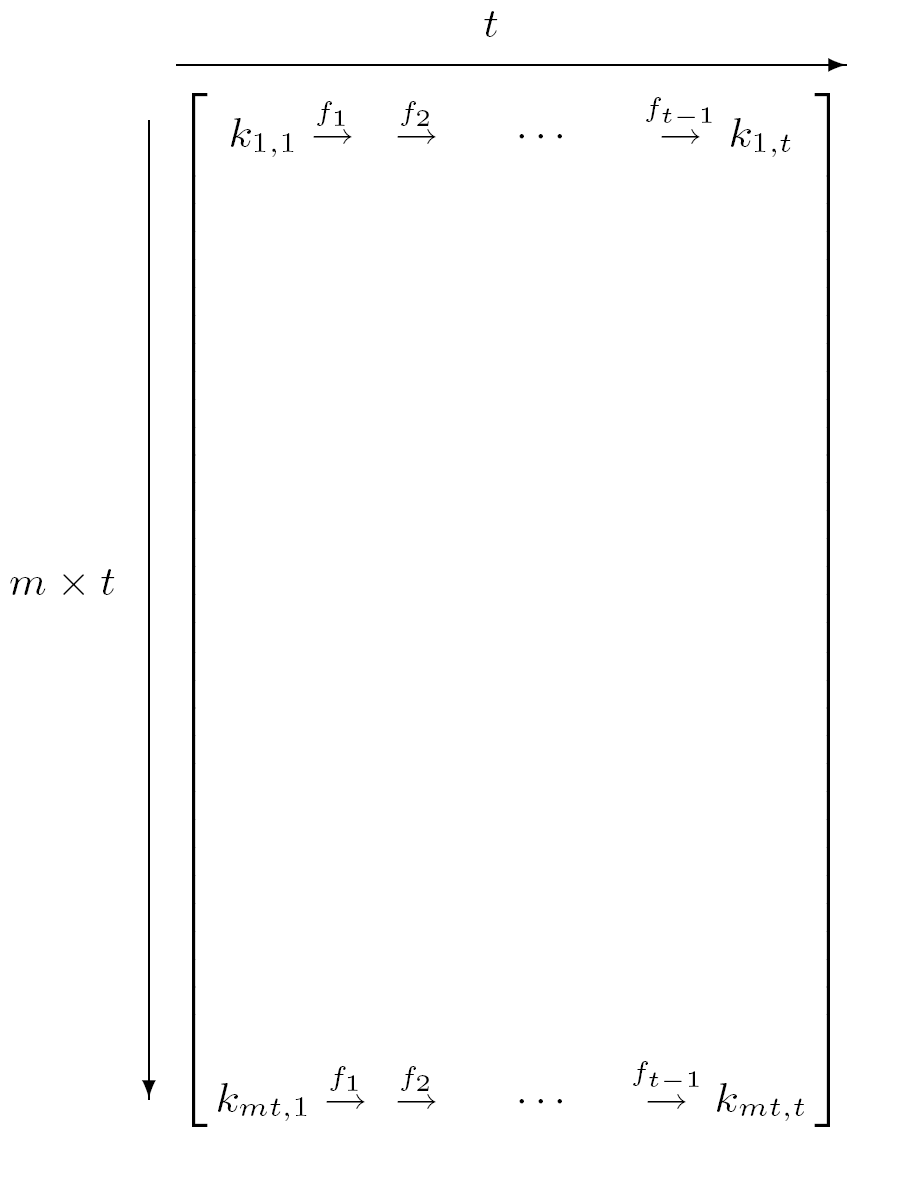
\includegraphics[width = 1.94in]{./figures/rainbow-table.PNG}
	\end{figure}

\end{column}
\end{columns}

\end{frame}

\begin{frame}{Rainbow table}

\begin{columns}
\begin{column}{5cm}
\footnotesize{
\begin{itemize}
	\item Precomputation phase: mapping functions \mbox{$f_1, f_2, \ldots , f_t$}, where $f_i(K) = R_i(E_{K}(P))$ for $1 \leq i \leq t$
	\item Only starting and end points are stored in hashtable
	\item Goal is to cover all possible keys, so $P$ = $mt^2$; $M$ = $mt$
	\item Attack phase: possibility of $C$ occurring in each column is checked
	\item Worst case attack time: $T$ = $0 + 1 + 2 + \cdots + (t-1) \approx t^2/2$
	
\end{itemize}}
\end{column}

\begin{column}{5cm}
	\begin{figure}[htp]
	\centering
	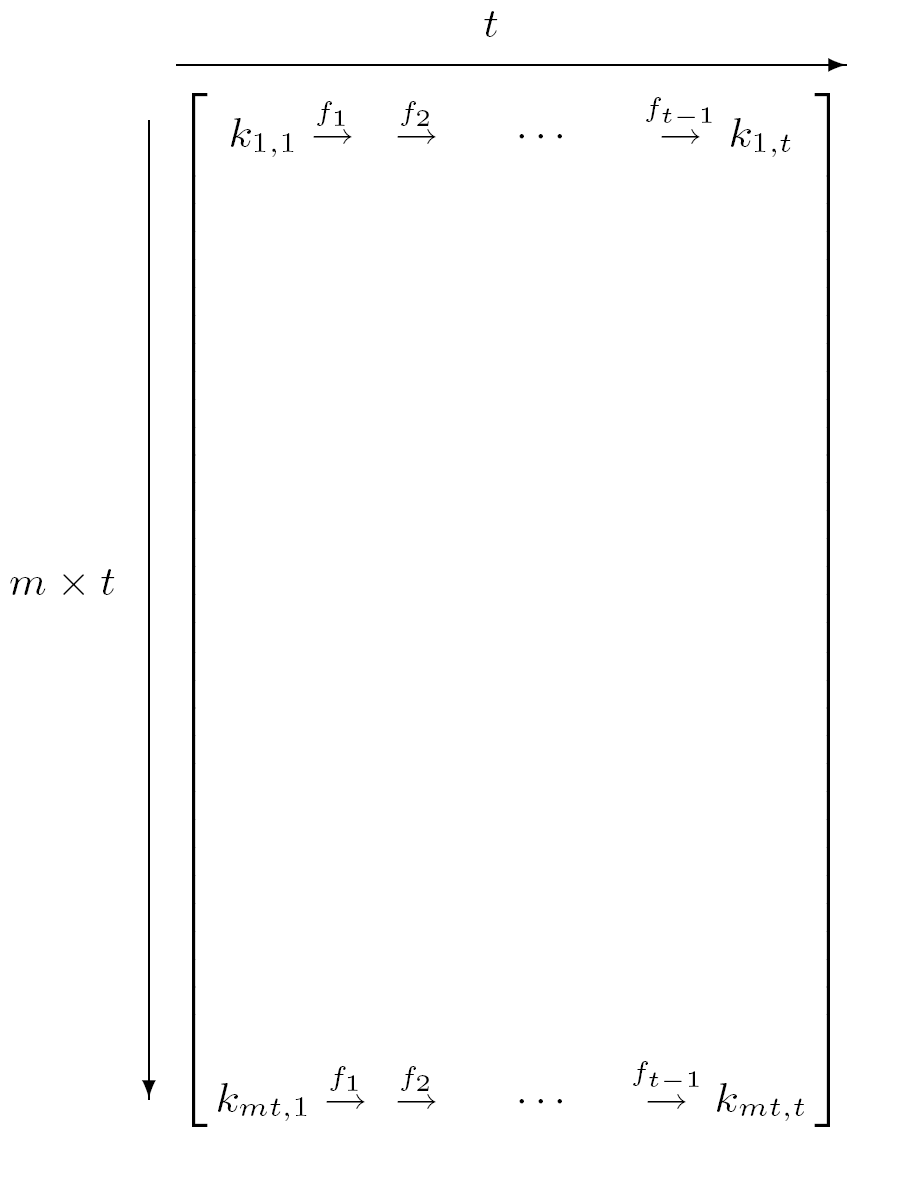
\includegraphics[width = 1.94in]{./figures/rainbow-table.PNG}
	\end{figure}

\end{column}
\end{columns}

\end{frame}

\subsection{Rainbow table for stream ciphers}

\begin{frame}{Modification for stream ciphers}
\begin{itemize}
\footnotesize{
	\item $P$ can be reduced due to availability of $D$ states in attack
	\item Tradeoff equation: $P \cdot D \geq 2^n$ or $Mt \cdot D \geq 2^n$
	\item Again, no dependency between precomputation phase parameters ($M,t$) and attack phase parameters ($D$)	
}\end{itemize}
\end{frame}

\subsection*{Implementation results}
\begin{frame}{Implementaton results}
\begin{columns}
\begin{column}{4cm}
\begin{itemize}
\scriptsize{
	\item Correct key is found atleast once for all combinations
	\item False keys also occur, but they can be supressed by using 56 bit prefixes
	\item Clearly, the number of false alarms is much less as compared with Hellman tables
}\end{itemize}
\end{column}
\begin{column}{7cm}
	\begin{figure}[htp]
	\centering
	\includegraphics[width = 2.7in]{./figures/table-tmdto-rainbow.PNG}
	\end{figure}
\end{column}	
\end{columns}
\end{frame}


\section{Conclusion}

\begin{frame}{Comparison of Hellman and rainbow tables}
\footnotesize{
\begin{itemize}
	\item Hellman tables for block cipher: $t$ tables, $t$ keys in each chain, $M$ chains
	\item Rainbow table for block cipher: 1 table, $t$ keys in each chain, $M$ chains
	\item Options for changing table structures for stream cipher in order to now satisfy $P \cdot D = 2^n$
	\begin{figure}[htp]
	\centering
	\includegraphics[width = 2.9in]{./figures/table-comparison-options.PNG}
	\end{figure}
	
\end{itemize}}
\end{frame}

\begin{frame}{Rainbow table}
\begin{columns}
\begin{column}{4cm}
\footnotesize{
\begin{itemize}
	\item Precomputation phase: mapping functions  \end{itemize}}
\end{column}
\begin{column}{6.5cm}
	\begin{figure}[htp]
	\centering
	\includegraphics[width = 2.7in]{./figures/table-comparison-results.PNG}
	\end{figure}
\end{column}
\end{columns}

\end{frame}

\begin{frame}{Concluding remarks}
\footnotesize{
\begin{itemize}
	\item 
\end{itemize}
}\end{frame}

\begin{frame}{Future work}
\footnotesize{
\begin{itemize}
	\item 
\end{itemize}
}\end{frame}

\begin{frame}
\begin{center}
	\HUGE{Thank you! }
\end{center}
\end{frame}

\end{document}


